% Define document class
\documentclass[%
 reprint,
%superscriptaddress,
%groupedaddress,
%unsortedaddress,
%runinaddress,
%frontmatterverbose, 
%preprint,
%preprintnumbers,
 nofootinbib,
%nobibnotes,
%bibnotes,
 amsmath,amssymb,
 aps,
 prd,
%prb,
%rmp,
%prstab,
%prstper,
%floatfix,
]{revtex4-2}
\usepackage[hidelinks]{hyperref}
\usepackage{graphicx}
% Begin!
\begin{document}

\preprint{APS/123-QED}

\title{BHPWAVE: An adiabatic gravitational waveform model for compact objects undergoing quasi-circular inspirals into rotating massive black holes}% Force line breaks with \\
%\thetaanks{A footnote to the article title}%

\author{Zachary Nasipak}
\affiliation{NASA Goddard Space Flight Center, 8800 Greenbelt Road, Greenbelt, Maryland, 20771, USA}
\email{zachary.nasipak@nasa.gov}

\date{\today}% It is always \today, today,
             %  but any date may be explicitly specified

\begin{abstract}
We present \texttt{bhpwave}: a new Python-based, open-source tool for generating the gravitational waveforms of stellar-mass compact objects undergoing quasi-circular inspirals into rotating massive black holes. These binaries, known as extreme-mass-ratio inspirals (EMRIs), are exciting millihertz gravitational wave sources for future space-based detectors. Relativistic models of EMRI gravitational wave signals are necessary to unlock the full scientific potential of these astrophysical sources, yet few open-source EMRI waveform models exist. To fill this void we built \texttt{bhpwave}, which uses the adiabatic approximation from black hole perturbation theory to rapidly construct gravitational waveforms based on the leading-order inspiral dynamics of the binary. Crucially \texttt{bhpwave} is the first open-source adiabatic model to produce waveforms for binaries with \emph{rotating} massive black holes, opening a new dimension of parameter space for astrophysical investigation.
\end{abstract}

%\keywords{Suggested keywords}%Use showkeys class option if keyword
                              %display desired
\maketitle

% Main body with filler text
\section{Introduction}
\label{sec:intro}

Extreme-mass-ratio inspirals (EMRIs) are binaries composed of a compact object with mass $\mu \sim 10 M_\odot$ inspiraling into a massive black hole with mass $M \sim 10^6 M_\odot$. They emit gravitational waves in the millihertz (mHz) band for months to years, making them promising sources for future space-based detectors, such as the Laser Interferometer Space Antenna (LISA) \cite{NASA11, ESA12}. The prolonged evolution and rich harmonic structure of an EMRI waveform communicates a wealth of information about the binary. Thus, we expect LISA to measure the masses, spins, and orbital characteristics of observed EMRIs with unprecedented accuracy \cite{BabaETC17}. These measurements will provide novel observations of massive black holes and their surrounding environments, while also facilitating high-precision tests of general relativity \cite{BerrETC19}. Extracting this information from an observed signal, however, will likely require subradian-accurate models of EMRI gravitational wave emission. 

Due to their small mass ratios $\epsilon = \mu/M \ll 1$, EMRIs are naturally modeled by black hole perturbation theory and the self-force formalism \cite{PounWard20}. Within this framework, the small body is treated as a perturbation to a background Kerr spacetime. The inspiral of the small body is then driven by a \emph{gravitational self-force} (GSF), which arises from the small body interacting with its own perturbation of the spacetime metric. The metric perturbations and the GSF are constructed perturbatively, order by order in $\epsilon$, to derive the dynamics and resulting gravitational wave emission of the binary. 

We can understand the relative impact of these self-forces on EMRI gravitational waveforms by expanding the phasing of the EMRI gravitational waveform $\Phi_\mathrm{GW}$ in powers of $\epsilon$ via a two-timescale analysis \cite{HindFlan08},
\begin{align}
\Phi_\mathrm{GW} = \frac{1}{\epsilon} \left[ \Phi_\mathrm{0PA} + \epsilon^{1/2} \Phi_\mathrm{res} + \epsilon \Phi_\mathrm{1PA} + O(\epsilon^2)\right].
\end{align}
The leading-order \emph{adiabatic} term\footnote{This term is also referred to as the post-0 adiabatic or 0PA term to remain consistent with the naming conventions of the sub-leading terms (e.g., $\Phi_\mathrm{1PA}$).} $\Phi_\mathrm{0PA}$ only depends on the time-averaged \emph{dissipative} first-order GSF, which drives the dissipation of energy and angular momentum from the system. The sub-leading post-1 adiabatic (1PA) piece $\Phi_\mathrm{1PA}$ depends on the remaining contributions from the first-order GSF and the time-averaged components of the second-order GSF. The half-order correction $\Phi_\mathrm{res}$ arises due to the presence of self-forced $r\theta$-resonances experienced by EMRIs undergoing eccentric and inclined inspirals \cite{FlanHind12}. EMRI gravitational models must, therefore, include the $\Phi_\mathrm{0PA}$, $\Phi_\mathrm{res}$, and $\Phi_\mathrm{1PA}$ effects in order to maintain sub-radian phase accuracy and enable the full scientific potential of future mHz gravitational wave observatories. 

Nonetheless purely adiabatic models---which only include $\Phi_\mathrm{0PA}$ in the gravitational wave phasing---may be suitable for detecting (but not characterizing) EMRI signals and are invaluable tools for developing data analysis pipelines for EMRI search and parametrization. They capture almost all of the phasing information and relativistic behavior of EMRI signals, making them powerful probes of astrophysical parameter space. The theoretical foundation and numerical calculation of adiabatic waveforms is also well understood, and has been performed for the most generic, eccentric, precessing EMRIs \cite{HughETC21}.

In practice, however, it is challenging to optimize adiabatic EMRI waveform calculations in order to make them efficient and accessible, so that they can be incorporated in large scale samplings of parameter space. Currently, only one open-source tool exists for producing adiabatic EMRI waveforms: the Fast EMRI Waveforms (FEW) Python package \cite{ChuaGallVall19, ChuaETC20, KatzETC20, KatzETC21}. While this tool is the gold standard for EMRI waveform models, particularly due to its ability to leverage GPUs, it is currently restricted to eccentric binaries with non-rotating black holes. Since we expect almost all astrophysical EMRIs to possess a rotating massive black hole, this model misses a crucial area of parameter space.

Therefore we introduce \texttt{bhpwave} [RTD link?] an open-source Python-based waveform generator that models the adiabatic dynamics and gravitational wave signals produced by a small body undergoing a quasi-circular\footnote{Quasi-circular refers to the fact that the particle is inspiraling so its motion is not circular, but at any moment of time its motion is tangent to a circular geodesic as described in Sec.~\ref{sec:adiabatic}. This is a consequence of the fact that in the adiabatic limit, circular orbits remain circular \cite{KennOri96, Kenn98}.} (non-eccentric) inspiral into a \emph{rotating} massive black hole. This code can model any binary with an initial orbital separation of $r_0 \leq 50 M$ and a massive black hole spin in the range $|a| \leq 0.995 M$. (See Sec.~\ref{sec:adiabatic} for exact definitions of $a$ and $r_0$.) Furthermore, the model supports any mass-ratio, though adiabatic waveform models are most relevant for $\epsilon \lesssim 10^{-4}$. By leveraging parallel computations across CPUs, \texttt{bhpwave} can evaluate years-long waveforms in milliseconds. Even on a standard laptop, waveform evaluations still complete within a few hundred milliseconds to a couple seconds.

A notable limitation of \texttt{bhpwave} is that it currently neglects the effects of eccentricity and precession.\footnote{In a frame where the massive black hole's angular momentum is held fixed, precession is instead described in terms of the inclination of the small body relative to the equatorial plane of the more massive black hole.} Nonetheless, while most observed EMRIs are expected to be highly eccentric \cite{GairETC04},  there are possible formation channels driven by accretion flow that circularize EMRI dynamics and align the orbital angular momentum with the massive black hole's spin \cite{PanLyuYang21}. Thus, \texttt{bhpwave} is applicable to these so-called ``wet-formation" EMRIs. 

Additionally, \texttt{bhpwave} does not provide the first adiabatic calculation of quasi-circular inspirals. These systems have long been studied in the literature \cite{Detw78, KennOri96, FinnThor00, Hugh00b, GralHughWarb16}. However, as aforementioned, it is challenging to implement an adiabatic model that is efficient, reliable, and accessible. Even when neglecting eccentricity, the inclusion of massive black hole spin presents a number of challenges that are less pronounced for binaries with non-spinning bodies, such as the larger range of radial separations accessible to spinning systems, the faster frequency evolution for more deeply bound orbits, and the higher mode content needed for modeling rapidly-rotating systems. By building upon the theoretical foundations described in the literature, our aim for \texttt{bhpwave} is to provide an efficient and accessible model that fills in this area of parameter space and provides an important stepping stone for developing more advanced models that incorporate all possible orbital effects.

To encourage the continued development of open-source adiabatic EMRI models, this paper outlines the theoretical and numerical foundations underpinning \texttt{bhpwave}. In Sec.~\ref{sec:adiabatic} we summarize the quasi-circular limit of the adiabatic approximation within the context of black hole perturbation theory to establish methods and notation. In Sec.~\ref{sec:bhpwave} we outline how \texttt{bhpwave} implements the quasi-circular adiabatic model, primarily through its three modules: \texttt{bhpwave.trajectory}, \texttt{bhpwave.harmonics}, and \texttt{bhpwave.waveform}. In Sec.~\ref{sec:numerical} we describe both the numerical routines used to generate the adiabatic data for \texttt{bhpwave} and the algorithms employed by \texttt{bhpwave} to generate quasi-circular inspirals, waveform harmonics, and gravitational signals. Additionally, we provide validation tests and model comparisons to verify the accuracy of \texttt{bhpwave}. To demonstrate the utility of \texttt{bhpwave}, in Sec.~\ref{sec:errors}, we use a toy problem test the impact of modeling errors on parameter biases for EMRI data analysis. Finally, we discuss further applications and possible extensions of \texttt{bhpwave} in Sec.~\ref{sec:conclusion}. For this paper we use the metric signature $(-+++)$, the sign conventions, where applicable, of \cite{MisnThorWhee73}, and units such that $c=G=1$.


\section{Adiabatic approximation}
\label{sec:adiabatic}

We provide a brief summary of the leading-order adiabatic approximation of a small body's quasi-circular inspiral into a rotating massive black hole. (For extensive discussions of the point-particle and adiabatic approximations see \cite{Hugh00b, Mino03, DrasHugh06, HughETC21} and references therein.) At zeroth-order the small body follows a circular, equatorial geodesic in Kerr spacetime (see \ref{sec:geo}). Due to its mass and motion, the small body excites gravitational radiation. At leading-order this radiation is captured by non-zero perturbations to the Weyl scalar $\psi_4$, which we construct via the Teukolsky equation (see \ref{sec:fluxes}). The resulting flux of energy dissipated via gravitational wave emission---which we compute from $\psi_4$---then drives the decay of the small body's orbital energy and thus the adiabatic inspiral (see \ref{sec:inspiral}). From this inspiral, we then construct the adiabatic gravitational waveform (see \ref{sec:waveform}).

\subsection{Circular, equatorial geodesics}
\label{sec:geo}

Consider a small body with mass $\mu$ orbiting in a Kerr spacetime with metric $g_{\mu\nu}$, which, in Boyer-Lindquist coordinates $(t,r,\theta,\phi)$, is defined by the line element
\begin{multline}
    ds^2 = -\left(1 - \frac{2Mr}{\Sigma} \right) dt^2 - \frac{4Ma r \sin^2\theta}{\Sigma} dtd\phi + \frac{\Sigma}{\Delta} dr^2 
    \\
    + \Sigma d\theta^2 + {\sin^2\theta}\left(r^2+a^2 + \frac{2Ma^2r\sin^2\theta}{\Sigma} \right) d\phi^2,
\end{multline}
where $a$ is the Kerr spin parameter, $M$ is the Kerr mass parameter, $\Delta = r^2 - 2Mr + a^2$, and $\Sigma = r^2+a^2\cos^2\theta$.

The mass $\mu$ follows a geodesic $z_p^\mu \doteq (t_p, r_p, \theta_p, \phi_p)$ that maintains a constant Boyer-Lindquist radius $r_p = r_0$ and is restricted to the equatorial plane $\theta_p = \pi/2$ (with respect to the angular momentum of the Kerr black hole). Due to the Killing symmetries of Kerr spacetime, this motion possesses three constants of motion: the orbital energy $u_t = - \mathcal{E}$, the $z$-component of the orbital angular momentum $u_\phi = \mathcal{L}_z$, and the Carter constant $\mathcal{Q} = Q_{\mu\nu} u^\mu u^\nu$, which are related to $a$ and $r_0$ by
\begin{subequations} \label{eqn:En}
\begin{align}
    \mathcal{E} &= \frac{1 - 2 v^2 \pm \hat{a} v^3}{\sqrt{1-3v^2\pm 2\hat{a}v^3}},
    \\
    \mathcal{L}_z &= \pm M  \frac{1 \mp 2 \hat{a} v^3 + \hat{a}^2 v^4}{v\sqrt{1-3v^2\pm 2\hat{a}v^3}},
    \\
    \mathcal{Q} &= 0,
\end{align}
\end{subequations}
where $\hat{a} \equiv a/M$, $v^2 = M/r_0$, and $+$ ($-$) refers to prograde (retrograde) orbits.

For circular orbits, the four-velocity $u^\alpha = dz_p^\alpha/d\tau \doteq (\omega_t, 0, 0, \omega_\phi)$ is constant along the geodesic, where $\tau$ is the proper time of the small body. The rates at which (Boyer-Lindquist) time and the azimuthal angle accumulate with $\tau$ are given by
\begin{subequations}
\begin{align}
    \omega_t &= \frac{g_{\phi\phi} \mathcal{E} + g_{t\phi}\mathcal{L}_z}{g_{t\phi}^2-g_{\phi\phi}g_{tt}} = \frac{1 \pm \hat{a} v^3}{\sqrt{1 - 3 v^2 \pm 2 \hat{a} v^3}},
    \\
    \omega_\phi &= -\frac{g_{t\phi} \mathcal{E} + g_{tt}\mathcal{L}_z}{g_{t\phi}^2-g_{\phi\phi}g_{tt}} = \pm \frac{v^3}{M\sqrt{1 - 3 v^2 \pm 2 \hat{a} v^3}},
\end{align}
\end{subequations}
respectively. Straightforward integration then yields
\begin{align*}
    t_p(\tau) &= \omega_t \tau,
    &
    r_p(\tau) &= r_0,
    &
    \theta_p(\tau) &= \frac{\pi}{2},
    &
    \phi_p(\tau) &= \omega_\phi\tau.
\end{align*}
Combining these results, we can re-express the evolution of the orbital phase in terms of coordinate time, $\phi_p(t) = \Omega_p t$, where the geodesic orbital frequency
\begin{equation} \label{eqn:OmegaOfR}
    \Omega_p = \frac{\omega_\phi}{\omega_t}
    = \pm \frac{v^3}{M(1 \pm \hat{a} v^3)}.
\end{equation}
Finally, the innermost stable circular orbit (ISCO) is defined in terms of the minimum radius
\begin{align}
    r_\mathrm{ISCO} &= 3 + z_2 \mp
    \sqrt{(3 - z_1)(3 + z_1 + 2z_2)},
    \\ \notag
    z_1 & = 1 + (1 - \hat{a}^2)^{1/3}
    \left((1-\hat{a})^{1/3} + (1 + \hat{a})^{1/3} \right),
    \\ \notag
    z_2 &= \sqrt{3 \hat{a}^2 + z_1^2},
\end{align}
and maximum frequency $M\Omega_\mathrm{ISCO} = r_\mathrm{ISCO}^{3/2}(M^{3/2} + \hat{a} r_\mathrm{ISCO}^{3/2})^{-1}$.

\subsection{Gravitational wave fluxes}
\label{sec:fluxes}

Next we consider how the small body's motion excites perturbations to the background spacetime. Using the Teukolsky formalism \cite{Teuk73}, we describe these perturbations in terms of the Weyl scalar $\psi_4$, which vanishes in an unperturbed Kerr spacetime and captures two of the ten gravitational degrees of freedom of the metric perturbation. Near infinity, these two degrees of freedom can be related to $h_+$ and $h_\times$ \cite{DrasHugh06}, the two polarizations of the gravitational strain, via
\begin{align} \label{eqn:psi4ToH}
    \psi_4 (r\rightarrow \infty) \simeq \frac{1}{2}(\ddot{h}_+ - i \ddot{h}_\times).
\end{align}
At adiabatic order, $\psi_4$ satisfies the spin-weight $s=-2$ Teukolsky equation (Eq.~(4.7) in \cite{Teuk73}) with a point-particle source (see Sec.~II of \cite{SasaTago03}). The solution is amenable to separation of variables in the frequency-domain, leading to the mode-sum representation
\begin{align} \label{eqn:psi4Modes}
    \psi_4 = \rho^{4} \sum_{j=2}^\infty \sum_{m=-j}^j R_{-2jm}(r) S_{-2jm}(\theta;\gamma) e^{im\phi} e^{-im\Omega_pt},
\end{align}
where $\rho = -(r-ia\cos\theta)^{-1}$, $S_{-2jm}(\theta;\gamma)$ is the spin-weighted spheroidal harmonic of spin-weight $s=-2$ and spheroidicity $\gamma=a m\Omega_p$ (which satisfies Eq.~(2.7) in \cite{TeukPres74}), and $R_{-2jm}(r)$ is the $s=-2$ radial Teukolsky solution (which satisfies Eq.~(3.12) in \cite{DrasHugh06}).

The spin-weighted spheroidal harmonics can be conveniently represented as a rapidly-converging series of spin-weighted spherical harmonics $Y_{s\ell m}$ \cite{Hugh00b},
\begin{align}
    S_{sjm}(\theta, \gamma)e^{im\phi} = \sum_{\ell=\ell_\mathrm{min}}^\infty b_{sjm}^\ell(\gamma) Y_{s\ell m}(\theta,\phi),
\end{align}
where $\ell_\mathrm{min}=\mathrm{max}[|m|,|s|]$. This decomposition is particularly useful because it allows us to reproject $\psi_4$ onto an angular basis that is independent of frequency,
\begin{align} \label{eqn:psi4LModes}
    \psi_4 = \rho^{4} \sum_{\ell=2}^\infty \sum_{m=-\ell}^\ell X_{-2\ell m}(r) e^{-im\Omega_pt} Y_{-2\ell m}(\theta, \phi),
\end{align}
where
\begin{align} \label{eqn:XfromR}
    X_{-2\ell m}(r) \sum_{j=\ell_\mathrm{min}}^\infty b_{-2jm}^\ell(\gamma)R_{-2jm}(r).
\end{align}
Furthermore, the spin-weighted spherical harmonics form a complete and orthonormal set of basis functions of the unit sphere (for the same value of spin-weight),
\begin{align}
    \int Y_{s\ell m} \bar{Y}_{s\ell'm'} d\Omega = \delta_{l l'} \delta_{m m'}.
\end{align}

%In general, the spin-weighted spheroidal harmonics satisfy,
% \begin{multline}
%     \Bigg[\frac{1}{\sin\theta}\frac{d}{d\theta}\left(\sin\theta \frac{d}{d\theta} \right)
%     - \bigg(\gamma^2\sin^2\theta -2m\gamma -s
%     \\
%     +\frac{(m+s\cos\theta)^2}{\sin^2\theta}
%     +2\gamma s\cos\theta -\lambda_{sjm\gamma} \bigg) \Bigg]S_{sjm\gamma} = 0,
% \end{multline}
% with eigenvalue $\lambda_{sjm\gamma}$. Therefore, we restrict ourselves to the case $S_{-2jm} = S_{-2jm(\gamma=am\Omega_p)}$. 

% For general spin-weight $s$ and frequency $\omega$, the radial Teukolsky solution satisfies
% \begin{align}
%     \left[\Delta^{-s} \frac{d}{dr} \left(\Delta^{s+1} \frac{d}{dr}  \right)
% 	+ V_{sjm\omega}(r)\right]R_{sjm\omega}(r) = T_{sjm\omega}(r)
% \end{align}
% where
% \begin{align}
%     V_{sjm\omega} &= \frac{K^2+4i(r-M)K}{\Delta}-8i\omega r - \lambda_{sjm(a\omega)},
% \end{align} 
% $K = (r^2+a^2)\omega - ma$, and the source term $T_{sjm\omega}$ is given in \cite{Teuk73}. 

For our point-particle source on a circular geodesic, the radial mode function $R_{-2jm}(r)$ have the asymptotic forms
\begin{subequations} \label{eqn:asympR}
\begin{align}
    R_{-2jm}(r\rightarrow r_+) &\simeq Z^\mathcal{H}_{-2jm} \Delta^{2} e^{-im k_p r_*},
    \\ 
    R_{-2jm}(r\rightarrow \infty) &\simeq Z^\mathcal{I}_{-2jm} r^{3} e^{+im\Omega_p r_*},
\end{align}
\end{subequations}
where $k_p = \Omega_p - \Omega_+$, $\Omega_+ = a/(2Mr_+)$, and the tortoise coordinate $r_*$ is given by the differential relation $dr_*/dr = (r^2+a^2)/\Delta$.
The amplitudes $Z^\mathcal{H/I}_{-2jm}$ are often referred to as \emph{Teukolsky amplitudes} and are constructed via the standard Green's function method, also known as the method of variation of parameters (see Sec.~III\,A in \cite{HughETC21} or \cite{DrasHugh06} for further details). From \eqref{eqn:XfromR}, we see that $X_{-2\ell m}$ then possesses the same asymptotic behavior as $R_{-2\ell m}$ in \eqref{eqn:asympR} but with modified amplitudes
\begin{align}
    Z^\mathrm{H/I}_{-2jm} \rightarrow X^\mathrm{H/I}_{-2\ell m} = \sum_{j=\ell_\mathrm{min}}^\infty b^\ell_{-2jm}(\gamma) Z^\mathrm{H/I}_{-2jm}.
\end{align}
As a final note, because $Z^\mathrm{H/I}_{-2jm}$ and  $X^\mathrm{H/I}_{-2\ell m}$ depend on the source motion, we can parametrize both amplitudes in terms of the orbital constants, e.g., $X^\mathcal{H/I}_{-2\ell m}= {X}^\mathcal{H/I}_{-2ell m}(\Omega_p; a)$.

Upon obtaining $\psi_4$, we can then calculate the flux of energy that this radiative field carries away to infinity $\dot{E}^\mathcal{I}$ and the flux radiated down the black hole horizon $\dot{E}^\mathcal{H}$ \cite{TeukPres74}, 
\begin{subequations} \label{eqn:fluxes}
\begin{align}
    \dot{E}^\mathcal{I} &= \frac{1}{4\pi} \sum_{jm} \alpha_{jm}^\infty {|Z^\mathcal{I}_{-2jm}|^2},
    \\
    \dot{E}^\mathcal{H} &= \frac{1}{4\pi} \sum_{jm} \alpha_{jm}^\mathcal{H} {|Z^\mathcal{H}_{-2jm}|^2},
\end{align}
\end{subequations}
where 
\begin{align*}
    \alpha_{jm}^\mathcal{I} &= \frac{1}{m^2\Omega_p^2},
    \\
    \alpha_{jm}^\mathcal{H} &= \frac{256m^2 k_p\Omega_p(2Mr_+)^5(m^2k_p^2+4\epsilon^2)(m^2k_p^2+16\epsilon^2)}{|C_{2jm}|^2},
\end{align*}
$\epsilon = (r_+ - M)/(2Mr_+)$, and the Teukolsky-Starobinsky constant is given by
\begin{align} 
    |C_{2jm}|^2 &=\Lambda_{2j m }^2(\Lambda_{2j m }-2)^2
    \\ \notag
    & \quad + 8 a m^2 \Omega_p(1 - a \Omega_p)(\Lambda_{2j m }-2)(5\Lambda_{2j m }-4)
    \\ \notag
    & \quad \quad
    +48 (a m \Omega_p)^2[4(\Lambda_{2j m }-1)+3m(1- a \Omega_p)].
\end{align}
Note that the Chandrasekhar eigenvalue $\Lambda_{sjm} = \lambda_{sjm} + s(s+1)$ is invariant under the interchange $s\rightarrow -s$ \cite{Chan83}.
The angular momentum fluxes are then related to the energy fluxes by $\dot{L}_z^{\mathcal{I}/\mathcal{H}} = \Omega^{-1} \dot{E}^{\mathcal{I}/\mathcal{H}}$, leading to the total gravitational wave fluxes
\begin{align}
    \dot{E}^\mathrm{GW} &= \dot{E}^\mathcal{I} + \dot{E}^\mathcal{H},
    &
    \dot{L}_z^\mathrm{GW} &= \dot{L}_z^\mathcal{I} + \dot{L}_z^\mathcal{H}.
\end{align}

\subsection{Adiabatic quasi-circular inspirals}
\label{sec:inspiral}

Due to gravitational {radiation-reaction}, the small body does not remain on a circular geodesic. The binary \emph{radiates} gravitational waves and the small body \emph{reacts} to the radiative losses of energy and angular momentum by undergoing a quasi-circular inspiral into the rotating massive black hole. We can parametrize this motion in terms of the time-evolving orbital energy ${E}(t)$ and orbital phase $\Phi(t)$ of the inspiraling body, which at leading order is given by the equations of motion \cite{PounWard20,HughETC21},
\begin{align} \label{eqn:eom}
    \frac{d {E}}{dt} &= \epsilon \mathcal{F}_t + O(\epsilon^2),
    &
    \frac{d\Phi}{dt} &= \Omega + O(\epsilon).
\end{align}
Because $\dot{E} \sim \epsilon$, the orbital energy evolves gradually and the evolution can be understood in terms of the \emph{osculating geodesics} method \cite{GairETC11}. At any time $t_0$, the motion is approximately tangent to a geodesic with energy $E(t_0) \approx \mathcal{E}$ and frequency $\Omega(t_0) \approx \Omega_p$. The small body then evolves from geodesic to geodesic based on its gravitational wave emission until the body approaches the ISCO, at which point the approximation breaks down and we end the evolution.

In effect, at leading order we can express the orbital frequency $\Omega$ in terms of the orbital energy ${E}$ using Eqs.~\eqref{eqn:En} and \eqref{eqn:OmegaOfR}, but with $\mathcal{E}$ and $\Omega_p$ replaced by $E$ and $\Omega$, respectively. Furthermore, the forcing term $\mathcal{F}_t$ is constructed using flux-balance arguments \cite{Mino03, Galt82, QuinWald99}: the loss of orbital energy is balanced by the energy flux due to gravitational wave radiation produced by a point-particle on a circular geodesic $\dot{E}^\mathrm{GW}$, leading to the relation $\epsilon \mathcal{F}_t = - \dot{E}^\mathrm{GW}$. 

As seen from Eq.~\eqref{eqn:eom}, the time it takes the system to undergo this inspiral scales with the radiation reaction timescale $T_\mathrm{insp} \sim T_\mathrm{rr} = M \epsilon^{-1}$. Similarly, the total accumulated phase scales like $\Delta\Phi_\mathrm{insp} \sim \epsilon^{-1}$.

\subsection{Time domain adiabatic waveform}
\label{sec:waveform}

After determining the adiabatic inspiral of the smaller body, we generalize \eqref{eqn:psi4LModes}---our geodesic expression for $\psi_4$---by once again leveraging the fact that at any moment of time the motion is approximately tangent to a geodesic. Consequently, the field amplitudes slowly evolve with frequency and time $X^\mathcal{H/I}_{-2\ell m}(\Omega_p; a) \rightarrow X^\mathcal{H/I}_{-2\ell m}(\Omega(t); a)$, while the field's phase rapidly accumulates in proportion to the orbital phase $\Omega_p t \rightarrow \Phi(t)$. As a result, the adiabatic waveform $h = h_+ - i h_\times$ takes the form
\begin{align} \label{eqn:adiabaticWaveform}
    h(u,r,\theta,\phi) = \frac{\mu}{r}\sum_{\ell m} B_{\ell m}(u) Y_{-2\ell m}(\theta, \phi) e^{-im\Phi(u)},
\end{align}
where, assuming $r \gg M$, the waveform amplitudes are given by
\begin{align} \label{eqn:amplitude}
    B_{\ell m}(u) = -2\frac{X_{-2\ell m}^\mathcal{I}( \Omega(u);a)}{m^2\Omega^2(u)} = A_{\ell m} e^{i \psi_{\ell m}}.
\end{align}
For later convenience we introduce $A_{\ell m} = |B_{\ell m}|$, the magnitude of the waveform amplitudes, and $\psi_{\ell m}$, the phase of the complex amplitudes, both of which depend on $\Omega(u)$ and $a$. Furthermore, rather than using the conventions of \cite{KatzETC21,HughETC21}, we follow \cite{PounWard20} and parametrize the adiabatic waveform in terms of the outgoing time-coordinate $u=t-r_*$. As a result, if we hold the orbital constants and frequencies fixed, \eqref{eqn:adiabaticWaveform} reduces to a geodesic ``snapshot'' waveform obtained via \eqref{eqn:psi4ToH} and \eqref{eqn:psi4LModes}. In practice, when implementing \eqref{eqn:adiabaticWaveform} in \texttt{bhpwave}, we replace $u$ with Boyer-Lindquist time $t$ to match the FEW model (which is described by (10) in \cite{KatzETC21}). This is equivalent to parametrizing all of our waveforms with an initial time $t_0 = r_*$.

\subsection{Frequency domain waveforms}

The amplitude and phase decomposition of \eqref{eqn:adiabaticWaveform} makes it particularly straightforward to represent our waveforms in the frequency domain via the stationary phase approximation \cite{HughETC21},
\begin{align}
    \tilde{h}(f) &= \int_{-\infty}^\infty h(t) e^{2\pi i f t} dt,
    \\ \notag
    & \approx \frac{\mu}{r}\sum_{\ell m} \tilde{B}_{\ell m}(f) Y_{-2\ell m}(\theta, \phi) e^{i[2\pi f t_p(f)- m\Phi(t_p(f))]},
\end{align}
where
\begin{align} \label{eqn:fourierAmplitude}
    \tilde{B}_{\ell m}(f) \approx \sqrt{\frac{2\pi}{i m \dot{\Omega}[t_p(f)]}} {B}_{\ell m}(t_p(f)),
\end{align}
and $t_p(f)$ refers to the times at which the binary emits gravitational waves with frequency $f$. For each $(\ell, m)$-mode, time and frequency are approximately related by
\begin{align} \label{eqn:fourierPhase}
    2\pi f \approx m \dot{\Phi}(t) = m \Omega(t),
\end{align}
which we can invert to approximate $t_p(f)$ for individual harmonics. As explained in Appendix \ref{app:fourierPhase}, both \eqref{eqn:fourierAmplitude} and \eqref{eqn:fourierPhase} neglect terms related to $\dot{\psi}_{\ell m}$ and $\ddot{\psi}_{\ell m}$, which introduces an $O(\epsilon)$ error to the phase and an $O(\epsilon^{1/2})$ error to the amplitude. Since the amplitudes scale as $\tilde{B}_{\ell m}(f) \sim 1/\sqrt{\epsilon}$, it is safe to neglect these terms for small mass-ratios.

\section{Solar system barycenter waveforms}

Up to this point, waveforms have been constructed in the source frame, with our Boyer-Lindquist coordinate system centered on the massive black hole. To get the observed waveform in the solar system barycenter (SSB) frame $h_\mathrm{SSB}$, we adopt the same conventions as the \textsc{FEW} model and make use of the transformation provided in \cite{KatzETC21}. In this frame, 
a generic EMRI system is parametrized by the 12 intrinsic parameters $(\mu, M, a, \vec{a}_2, p_0, e_0, x_0, \Phi_{r0}, \Phi_{\theta 0}, \Phi_{\phi 0})$---where $\vec{a}_2$ is the spin-vector of the smaller body; $p_0$, $e_0$, and $x_0$ are respectively the initial semi-latus rectum, orbital eccentricity, and projection of the orbital inclination; and $\Phi_{r0}$, $\Phi_{\theta 0}$, $\Phi_{\phi 0}$ are respectively the initial radial, polar, and azimuthal phases---and the 5 extrinsic parameters $(d_L, q_S, \phi_S, q_K, \phi_K)$---where $d_L$ is the luminosity distance to the source EMRI, $q_S$ and $\phi_S$ are the polar and azimuthal sky positions of the source, and $q_K$ and $\phi_K$ are the polar and azimuthal angles defining the orientation of the massive black hole's axis of rotation. In our simplified quasi-circular setup, five of the intrinsic parameters are constrained to the values $\vec{a}_2 = 0$, $e_0 = 0$, $x_0 = 1$, $\Phi_{r0} = \Phi_{\theta 0} = 0$, while two of the remaining free parameters are given by $\Phi_{\phi 0} = \Phi(0)$ and $p_0 = r_0$.

The extrinsic parameters are related to Boyer-Lindquist $(r,\theta, \phi)$ via
\begin{subequations}
    \begin{align}
        r &= d_L,
        \\
        \cos\theta &= - \cos q_S\cos q_K
        \\ \notag
        & \qquad \quad -\sin q_S \sin q_K \cos(\phi_K - \phi_S),
        \\
        \phi &= -\frac{\pi}{2}.
    \end{align}
\end{subequations}
The frame transformation also rotates the strain amplitudes by the polarization angle $\psi$. As a result, $h_\mathrm{SSB}$ is related to $h$, the strain in the source frame, via
\begin{align}
    h_\mathrm{SSB} = e^{i\psi} h = \frac{D_\psi^2}{|D_\psi|^2} h,
\end{align}
where $D_\psi$ is given by
\begin{multline}
    D_\psi = \cos q_S \sin q_K \cos(\phi_K - \phi_S)
    \\ 
     - \sin q_S\cos q_K +i \sin q_K \sin(\phi_K - \phi_S).
\end{multline}

\section{Numerical methods}
\label{sec:numerical}

\subsection{Fluxes and inspiral}

To simplify the calculation of our inspirals, we introduce the dimensionless and rescaled orbital quantities
\begin{align}
    \check{t} &= \frac{\mu t}{M^2},
    &
    \check{\Phi} &= \frac{\mu \Phi}{M},
    &
    \hat{\Omega} &= M \Omega,
    &
    \hat{a} &= \frac{a}{M}.
\end{align} 
A hat represents a quantity that is made dimensionless, while a check represents a quantity that is dimensionless and scaled by the mass ratio. We then reparametrize the equations of motion in terms of the (dimensionless) orbital frequency, yielding
\begin{subequations}
\begin{align}
    \frac{d\check{t}}{d\hat{\Omega}} &= \left[\partial_{\mathcal{E}}\hat{\Omega}(\hat{\Omega}; \hat{a}) {\mathcal{F}}_t(\hat{\Omega}; \hat{a})\right]^{-1},
    \\
    \frac{d\check{\Phi}}{d\hat{\Omega}} &= \hat{\Omega} \left[\partial_{\mathcal{E}}\hat{\Omega}(\hat{\Omega}; \hat{a}) {\mathcal{F}}_t(\hat{\Omega}; \hat{a})\right]^{-1}.
\end{align} 
\end{subequations}
The Jacobian $\partial_{\mathcal{E}}\hat{\Omega}$ is analytically obtained from \eqref{eqn:En} and \eqref{eqn:OmegaOfR}, while we construct ${\mathcal{F}}_t$ numerically via \eqref{eqn:fluxes}.

In this form, the equations of motion no longer depend on the masses of the binary, just the dimensionless orbital frequency and dimensionless Kerr spin parameter.
Therefore, we can pre-compute the rescaled trajectories $\check{t}(\hat{\Omega}; \hat{a})$ and $\check{\Phi}(\hat{\Omega}; \hat{a})$ and store them on a numerical grid spanning the domain of $\hat{a}$ and $\hat{\Omega}$. This allows us to construct bicubic spline interpolants to represent the trajectories. We can then rapidly evaluate the numerical interpolants to get any quasi-circular inspiral within our domain. 

For this work, we set the boundaries of our grid at $\hat{a} \in [-\hat{a}_\mathrm{max}, +\hat{a}_\mathrm{max}]$ and $\hat{\Omega} \in [\hat{\Omega}_\mathrm{min}, \hat{\Omega}_\mathrm{ISCO}]$ with $\hat{a}_\mathrm{max} = 0.9999$ and $\hat{\Omega}_\mathrm{min} = 2\times 10^{-3}$ (which corresponds to $r_0 \approx 50 M$). This domain is plotted in Fig.~\ref{fig:domain}, highlighting the particularly strong dependence of the lower frequency boundary $\hat{\Omega}=\hat{\Omega}_\mathrm{ISCO}$ on the black hole spin, which presents a challenge when sampling this space. Furthermore, as shown in Figure \ref{fig:temp}, $\check{t}$ and $\check{\Phi}$ accumulate quickly as $\hat{\Omega} \rightarrow \hat{\Omega}_\mathrm{ISCO}$ and $\hat{a} \rightarrow 1$. Therefore, a simple uniform sampling in $\hat{a}$ and $\hat{\Omega}-\hat{\Omega}_\mathrm{ISCO}$ could lead to substantial errors in our interpolating functions due to the large magnitudes of the higher-order derivatives with respect to $\hat{a}$ and $\hat{\Omega}$.

\begin{figure}
    \centering
    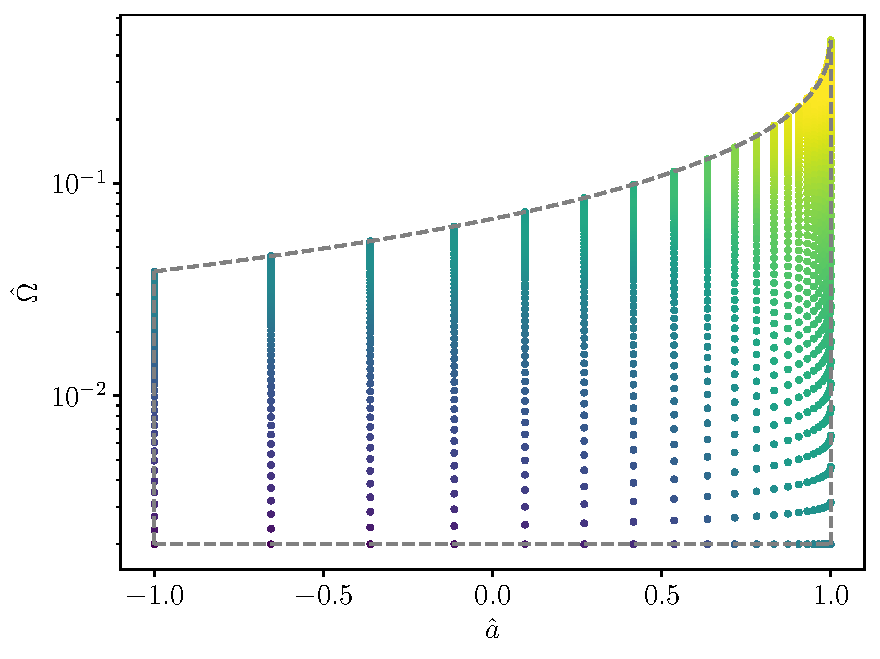
\includegraphics[width=0.95\columnwidth]{figures/domain_sampling.pdf}
    \caption{A $32\times 64$ grid in $(\beta, \alpha)$ mapped to the $(\hat{a}, \hat{\Omega})$ domain. Each dot represents a sampled point in the parameter space. These points are equally-spaced in $\alpha$ and in $\beta$, but cluster around $\hat{\Omega} = \hat{\Omega}_\mathrm{ISCO}$ and $\hat{a} = \hat{a}_\mathrm{max}$. The shading of each point reflects the relative density of points in the $(\hat{a}, \hat{\Omega})$ domain.}
    \label{fig:domain}
\end{figure}

Therefore, we aim to construct a parametrization that mitigates the errors in our numerical interpolations of the inspiral trajectories. We first ameliorate the rapid growth in time and phase by rescaling $\check{t}$ and $\check{\Phi}$ by their leading post-Newtonian behavior, as shown in Fig.~\ref{fig:tempa}. Next, motivated by post-Newtonian and near-extremal expansions of the orbital quantities, we introduce the parameters $x = \hat{\Omega}^{1/3}$ and $\chi = (1 - \hat{a})^{1/3}$, leading to the improved behavior in Fig.~\ref{fig:tempb}. In Fig.~\ref{fig:tempc} we plot the variation in $\check{t}$ and $\check{\Phi}$ with respect to the final parameters,
\begin{align} \label{eqn:params}
    \alpha^2 &= \frac{x_\mathrm{ISCO}-x}{x_\mathrm{ISCO}-x_\mathrm{min}},
    &
    \beta^2 &= \frac{\chi-\chi_-}{\chi_+-\chi_-},
\end{align}
where $x_\mathrm{min} = \Omega_\mathrm{min}^{1/3}$, $x_\mathrm{ISCO} = \Omega_\mathrm{ISCO}^{1/3}$, and $\chi_\pm = (1 \pm a_\mathrm{max})^{1/3}$. We square the left-hand side of \eqref{eqn:params} to further smooth out the behavior near the ISCO frequency and maximum spin values.

After choosing this parametrization, we solve for the fluxes $\dot{E}^\mathrm{GW}$ and precompute $\mathcal{F}_t$ on a fixed $129 \times 257$ equally-spaced grid in in $\beta \times \alpha$. These sampling points are mapped to $[a, \Omega]$ domain in Fig.~\ref{fig:domain}. This illustrates the concentration of sampling points towards the ISCO and near-extremal spins. 

For \texttt{bhpwave}, we produced a $129 \times 257$ regularly-spaced grid in $\beta \times \alpha$. These sampling points are mapped to $[a, \Omega]$ domain in Fig.~\ref{fig:domain}. This illustrates the concentration of sampling points towards the ISCO and near-extremal spins. 

Trajectory data are then precomputed on this grid. This data is compiled into bicubic spline interpolants for $\check{t}$, $\check{\Phi}$, $\check{\Phi}$ when \texttt{bhpwave} is loaded.

\subsection{Mode amplitudes and selection}

Similar to the trajectories, we presample the waveform amplitudes

\subsection{Waveform evaluation}

\subsection{Self-consistent validation tests}

\subsection{Model comparison}

\section{bhpwave}
\label{sec:bhpwave}

Our waveform model \texttt{bhpwave} is implemented through three Python modules: a trajectory module \texttt{bhpwave.trajectory} that generates goedesics and inspirals, a harmonic module \texttt{bhpwave.harmonics} described in Sec.~\ref{sec:harm}, and a waveform module \texttt{bhpwave.waveform} described in Sec.~\ref{sec:wave}.

\subsection{Trajectory module}
\label{sec:traj}

The trajectory module \texttt{bhpwave.trajectory} is separated into two submodules: 
\begin{enumerate}
    \item \texttt{bhpwave.trajectory.geodesic}
    \item \texttt{bhpwave.trajectory.inspiral}
\end{enumerate}
The geodesic module implements the equations of Sec.~\ref{sec:geo} and their derivatives with respect to the orbital parameters. The inspiral module constructs bicubic splines of pre-computed inspiral trajectories 

\subsection{Harmonics module}
\label{sec:harm}

The harmonics module \texttt{bhpwave.harmonics} is separated into two submodules: 
\begin{enumerate}
    \item \texttt{bhpwave.trajectory.swsh}
    \item \texttt{bhpwave.trajectory.amplitudes}
\end{enumerate}

\subsection{Waveform module}
\label{sec:wave}

The waveform module \texttt{bhpwave.waveform} is the parent module for computing 

\section{Assessing modeling errors}
\label{sec:errors}

\section{Conclusion}
\label{sec:conclusion}

\appendix

\section{Approximations of the frequency domain waveforms}
\label{app:fourierPhase}

Note that in our case, the stationary phase approximation is an asymptotic expansion with error $O(\epsilon^{1/2})$.

In the small mass-ratio limit, $M\dot{\Phi} = M\Omega \sim 1$ while $M \dot{\psi}_{\ell m} \sim \epsilon$. Therefore, neglecting the time-evolution of ${\psi}_{\ell m}$, we invert $f\approx m\Omega(t)/(2\pi)$ to approximate $t_p(f)$ for each $(\ell, m)$ mode. Similarly  At first glance, ignoring this $O(\epsilon)$ term may introduce an error of $O(1)$ in the values of $t_p$ and $\Phi(t_p)$, thus diminishing the phase accuracy of our frequency-domain waveform. However, these errors perfectly cancel, leading to an $O(\epsilon)$ error in the phasing, as explained in Appendix \ref{app:fourierPhase}.

Furthermore, when calculating $\tilde{B}_{\ell m}(f)$, we neglect any contribution from $\ddot{\psi}_{\ell m}$ in \eqref{eqn:fourierAmplitude}. We expect this approximation to introduce an $O(\epsilon)$ error relative to the leading-order behavior of $\tilde{B}_{\ell m}(f) \sim 1/\sqrt{\epsilon}$, and therefore is safe to neglect in the small mass-ratio limit.

This can be seen by parametrizing the time and phase in terms of $\Omega$. Then $\Omega_f = \Omega(f) = \Omega_0 + \delta\Omega$ where $\Omega_0 = 2\pi f/m$ and $\delta\Omega \sim \epsilon$. The induced error in the phasing $\Psi(f) = 2\pi f t(\Omega_f) + \psi_{\ell m}(\Omega_f) - m\Phi(\Omega_f)$ for a fixed value of $f$ is then given by
\begin{align}
    \Psi(f) &=
    m\Omega_0 t(\Omega_0) + \psi_{\ell m}(\Omega_0) - m\Phi(\Omega_0) 
    \\ \notag
    & \qquad + \big[m\Omega_0 \partial_\Omega t(\Omega_0) + \partial_\Omega\psi_{\ell m}(\Omega_0) 
    \\ \notag
    & \qquad \qquad + m\partial_\Omega\Phi(\Omega_0)\big]\delta \Omega + O(\delta\Omega^2),
    \\
    &=
    m\Omega_0 t(\Omega_0) + \psi_{\ell m}(\Omega_0) - m\Phi(\Omega_0) 
    \\ \notag
    & \qquad + \big[m\Omega_0 \partial_\Omega t(\Omega_0) + \partial_\Omega\psi_{\ell m}(\Omega_0) 
    \\ \notag
    & \qquad \qquad + m\partial_\Omega\Phi(\Omega_0)\big]\delta \Omega + O(\delta\Omega^2),
\end{align}

\bibliography{parent}

\end{document}
